% GENERATED by mb5.paper_numbers from paper/figures/figures.tex (mb5.figures)
\begin{figure*}[t]
  \centering
  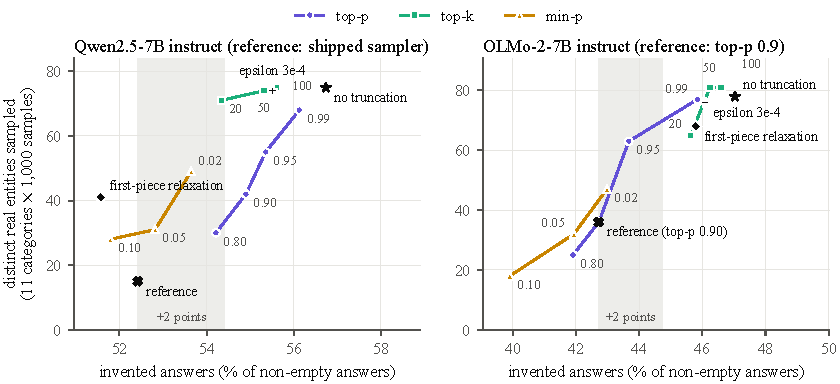
\includegraphics[width=\textwidth]{figures/fig6_frontier.pdf}
  \caption{The mitigation frontier (pilot, 11 categories, 1,000 samples per category and sampler). Each point is a sampler: distinct real member entities it produced against the share of answers that match no real member (``invented''; includes spelling variants and real names missing from Wikidata, see the hand audit). Lines join settings of one sampler family, labelled by their parameter. Shaded: within 2 points of the reference, the band gate G3 allowed. For Qwen, removing truncation raises distinct entities from 15 to 75 at 4.3 more points of invented answers.}
  \label{fig:frontier}
\end{figure*}
